\titre{1}
\theme{trigo}
\auteur{Nathan Scheinmann}
\niveau{1M}
\source{sesamath-1M-trigo}
\type{serie}
\piments{2}
\pts{}
\annee{2425}

\contenu{
\tcblower
Dans chaque cas, calculer la valeur arrondie au millième des longueurs manquantes.
\begin{tasks}(3)
	\task 
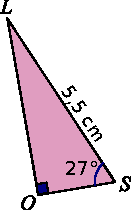
\includegraphics[scale=1]{../medias/1M/trigo/1M-exo-1-1}	
	\task 
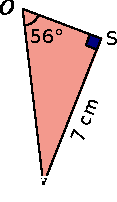
\includegraphics[scale=1]{../medias/1M/trigo/1M-exo-1-2}	
	\task 
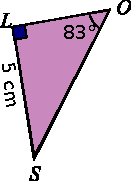
\includegraphics[scale=1]{../medias/1M/trigo/1M-exo-1-3}	
\end{tasks}
}
\correction{

}
